\documentclass[12pt,a4paper]{article}
\usepackage{geometry}
\usepackage[numbers]{natbib}
\usepackage{amssymb, amsmath}
\usepackage{graphicx}
\usepackage{grffile}
\graphicspath{{../Figures/}}
\usepackage{gensymb}
\usepackage[font=small]{caption}
\usepackage[utf8]{inputenc}
\usepackage[english]{babel}
\usepackage{fancyhdr}
\usepackage[raggedright]{titlesec}
\usepackage{subcaption}
\usepackage{multirow}
\usepackage{dirtytalk}
\usepackage{framed}
\usepackage[normalem]{ulem}
\usepackage[pdftex,breaklinks]{hyperref}
\hypersetup{
  colorlinks   = true, %Colours links instead of ugly boxes
  urlcolor     = green, %Colour for external hyperlinks
  linkcolor    = blue, %Colour of internal links
  citecolor   = red %Colour of citations
}


\begin{document}
\author{Katrina Ashton}


\pagestyle{fancy}
\fancyhf{}
\rhead{\thepage}
\lhead{u5586882}

\section{What I've done}
\begin{itemize}
  \item Updated background information and literature review sections of report based on your feedback. Still need to do some more work on the coordinate frames and find/make a better picture
  \item Worked on draft of PnP subsection of Background Information, added ICP subsection 
  \item Added PnP method
  \item Got ground truth working for new format (although the coordinate system is defined weirdly)
  \item Investigated Kabsch using inliers from EM and PnP, compared with MATLAB
  \item Thought about frames re: camera vs quad as defined by the Vicon. Tried to get my plotting function to do the trajectories in the same format as the ground truth (might need to think about this a bit more).
  \item Fixed up a few bugs (e.g. plotting inliers matches for Kabsch)
\end{itemize}

\section{Parts of report to look at}
\begin{itemize}
\item Background (section 4, page 8) the intro part before any subsections 
\end{itemize}

\section{Questions}
\begin{itemize}
\item 
\end{itemize}

\section{Comments}
\begin{itemize}
  \item The ground truth from the quadcopter has a different frame to the ground truth I got from the Vicon on the ground station. It also has -z and -y compared to how I naturally think about it (i.e. z up, x left, and y with RHR). Right now I'm plotting it in the way I think about the world frame, but I could be introducing errors.
  \item PnP and EM both seems to work pretty well (Figure \ref{f: quad3 trj}).
  \item Kabsch still isn't working with RANSAC or with inliers from either EM or PnP. The MATLAB Kabsch implementation also isn't working that well (using the PnP inliers seems a bit better than the EM inliers, but they're both pretty bad). (Figure \ref{f: quad3 kabsch}).
  \item I need to sort out my frames so that I can compare stuff with the ground truth properly.
  \item The orientation of the ground truth isn't changing, whereas the x-axis should always be pointing into the circle. Having a closer look at the Euler angles \ref{f: quad3 angles}, it seems like there might be a bit of a time delay on them (the trajectory starts at frame 700, where the yaw is still constant).
\end{itemize}

% \begin{figure}[h]
%   \centering
%   \includegraphics[width=60mm]{../data/quad1/rgb/1533792214.08.png}
%   \caption{Example RGB image, top of boxes is cut off}
%   \label{f: quad low rgb}
% \end{figure}

\begin{figure}[p]
\begin{subfigure}[t]{0.5\textwidth}
  \centering
    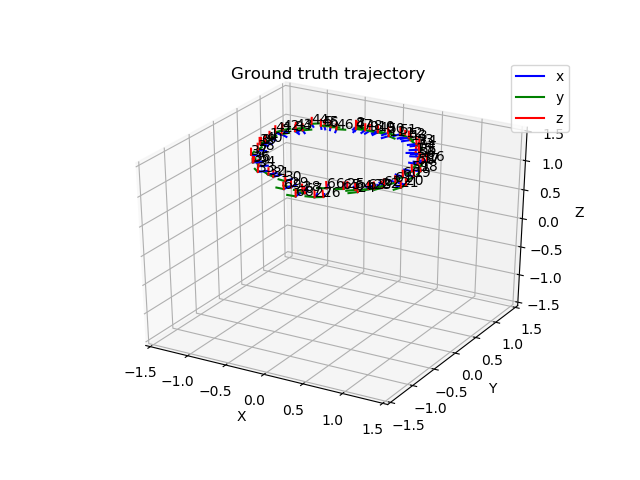
\includegraphics[width=80mm]{../quad/basic-reg-saves/rtrj_gt.png}
  \caption{Ground truth from Vicon}
  \end{subfigure}%
  ~
  \begin{subfigure}[t]{0.5\textwidth}
  \centering
    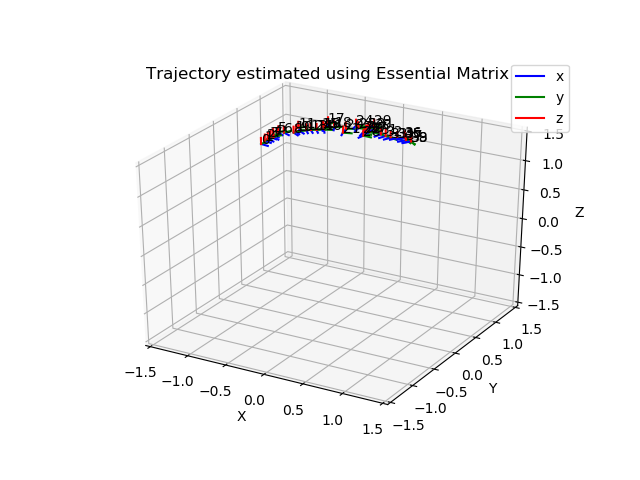
\includegraphics[width=80mm]{../quad/basic-reg-saves/rtrj_rgb.png}
  \caption{Estimated trajectory for Essential Matrix method, start at origin. Note axes scaling x4}
  \end{subfigure}
  \\
  \begin{subfigure}[t]{0.5\textwidth}
  \centering
    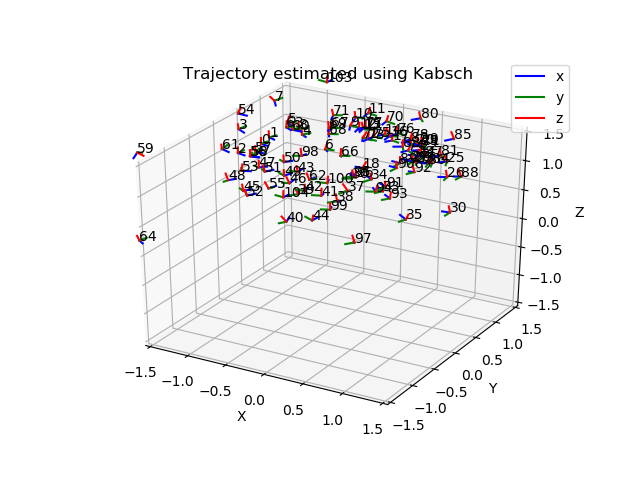
\includegraphics[width=80mm]{../quad/basic-reg-saves/rtrj_d.png}
  \caption{Estimated trajectory for Kabsch method, start at origin. Note axes scaling x2}
  \end{subfigure}%
  ~
  \begin{subfigure}[t]{0.5\textwidth}
  \centering
    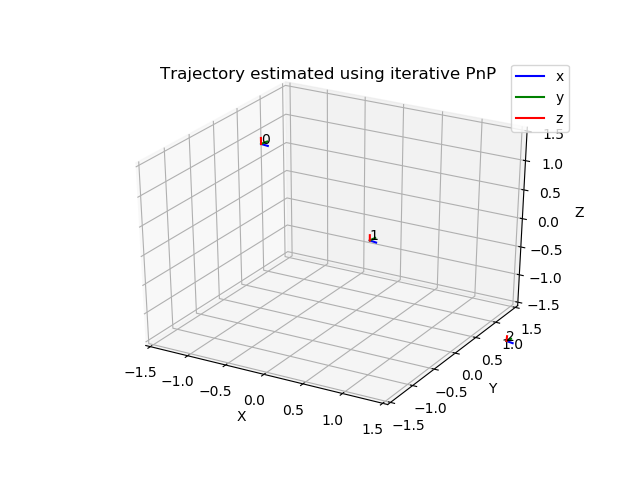
\includegraphics[width=80mm]{../quad/basic-reg-saves/rtrj_pnp.png}
  \caption{Estimated trajectory for PnP method, start at origin. Note axes scaling x2}
  \end{subfigure}
  \caption{Trajectory visualizations for third quad dataset}
  \label{f: quad3 trj}
\end{figure}

\begin{figure}[h]
\begin{subfigure}[t]{\textwidth}
  \centering
    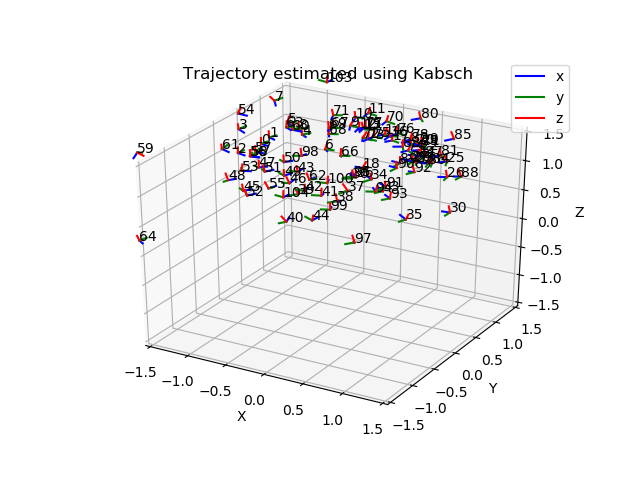
\includegraphics[width=80mm]{../quad/basic-reg-saves/rtrj_d.png}
  \caption{RANSAC Kabsch}
  \end{subfigure}%
  \\
  \begin{subfigure}[t]{0.5\textwidth}
  \centering
    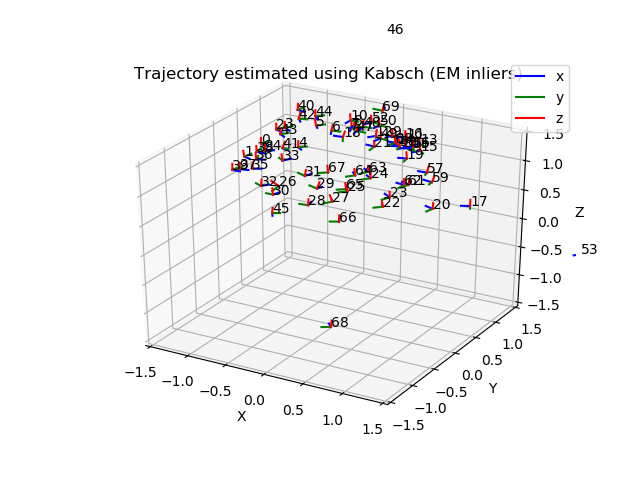
\includegraphics[width=80mm]{../quad/basic-reg-saves/rtrj_de.png}
  \caption{Kabsch with Essential Matrix inliers}
  \end{subfigure}%
  ~
  \begin{subfigure}[t]{0.5\textwidth}
  \centering
    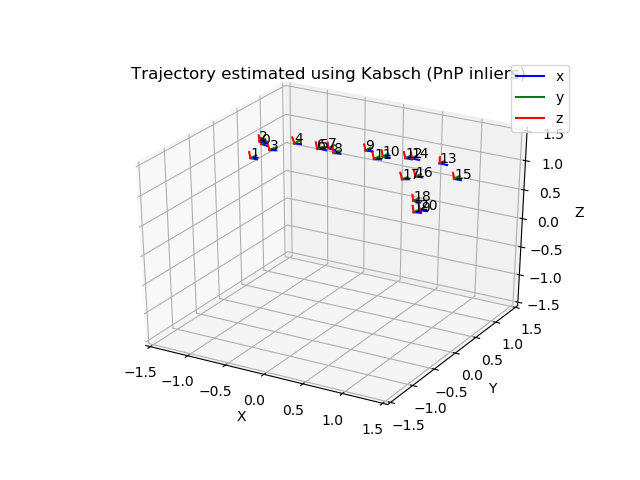
\includegraphics[width=80mm]{../quad/basic-reg-saves/rtrj_dp.png}
  \caption{Kabsch with PnP inliers}
  \end{subfigure}
  \\
  \begin{subfigure}[t]{0.5\textwidth}
  \centering
    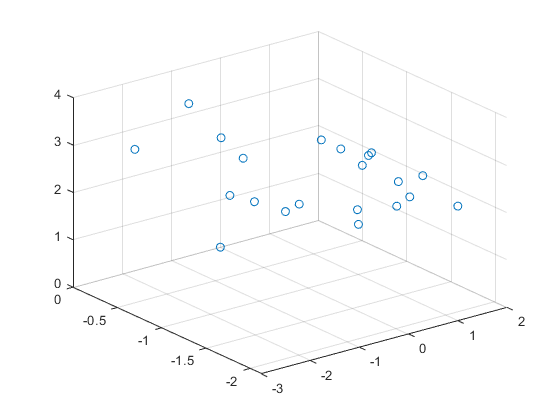
\includegraphics[width=80mm]{../quad/kabsch/unaligned.png}
  \caption{Kabsch with PnP inliers (MATLAB)}
  \end{subfigure}%  
  ~
  \begin{subfigure}[t]{0.5\textwidth}
  \centering
    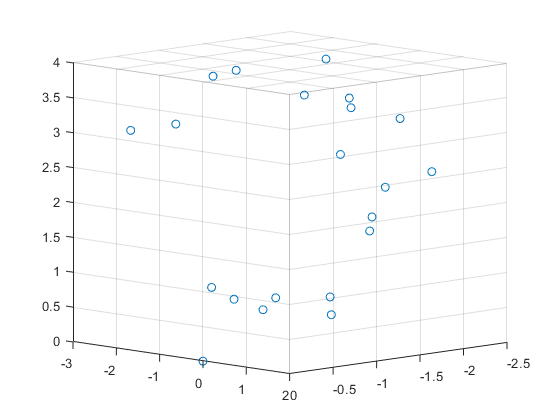
\includegraphics[width=80mm]{../quad/kabsch/aligned.png}
  \caption{Kabsch with PnP inliers (MATLAB), rotated to show shape}
  \end{subfigure}
  \caption{Trajectory visualizations for third quad dataset, Kabsch method with different inliers}
  \label{f: quad3 kabsch}
\end{figure}

\begin{figure}[h]
  \begin{subfigure}[t]{0.5\textwidth}
  \centering
    \includegraphics[width=80mm]{../quad/basic-reg-saves/angles_gt.png}
    \caption{All frames}
  \end{subfigure} %
  ~
  \begin{subfigure}[t]{0.5\textwidth}
    \includegraphics[width=80mm]{../quad/basic-reg-saves/angles_gt_aligned.png}
    \caption{Trajectory frames}
  \end{subfigure}
  \caption{Roll, pitch and yaw angles in ground truth for third quad dataset}
  \label{f: quad3 angles}
\end{figure}

% \begin{figure}[h]
%   \centering
%   \begin{subfigure}[t]{\textwidth}
%   \centering
%   \includegraphics[width=120mm]{../quad/matches/1533791935.37_essential.png}
%   \caption{Points used for Essential Matrix}
%   \end{subfigure}%
%   \\
%   \begin{subfigure}[t]{\textwidth}
%   \centering
%   \includegraphics[width=120mm]{../quad/matches/1533791935.37_kabsch.png}
%   \caption{Points used for Kabsch}
%   \end{subfigure}%
%   \caption{Matches after RANSAC (inliers) between two frames}
%   \label{f: matches}
% \end{figure}


\bibliographystyle{abbrvnat}
\bibliography{../Report/ENGN4217}

\end{document}